\documentclass[]{tufte-book}

% ams
\usepackage{amssymb,amsmath}

\usepackage{ifxetex,ifluatex}
\usepackage{fixltx2e} % provides \textsubscript
\ifnum 0\ifxetex 1\fi\ifluatex 1\fi=0 % if pdftex
  \usepackage[T1]{fontenc}
  \usepackage[utf8]{inputenc}
\else % if luatex or xelatex
  \makeatletter
  \@ifpackageloaded{fontspec}{}{\usepackage{fontspec}}
  \makeatother
  \defaultfontfeatures{Ligatures=TeX,Scale=MatchLowercase}
  \makeatletter
  \@ifpackageloaded{soul}{
     \renewcommand\allcapsspacing[1]{{\addfontfeature{LetterSpace=15}#1}}
     \renewcommand\smallcapsspacing[1]{{\addfontfeature{LetterSpace=10}#1}}
   }{}
  \makeatother

\fi

% graphix
\usepackage{graphicx}
\setkeys{Gin}{width=\linewidth,totalheight=\textheight,keepaspectratio}

% booktabs
\usepackage{booktabs}

% url
\usepackage{url}

% hyperref
\usepackage{hyperref}

% units.
\usepackage{units}


\setcounter{secnumdepth}{2}

% citations
\usepackage{natbib}
\bibliographystyle{apalike}

% pandoc syntax highlighting

% longtable
\usepackage{longtable,booktabs}

% multiplecol
\usepackage{multicol}

% strikeout
\usepackage[normalem]{ulem}

% morefloats
\usepackage{morefloats}


% tightlist macro required by pandoc >= 1.14
\providecommand{\tightlist}{%
  \setlength{\itemsep}{0pt}\setlength{\parskip}{0pt}}

% title / author / date
\title{Improving the Reproducibility of Experimental Data Recording and Pre-Processing}
\author{Brooke Anderson, Michael Lyons, Mercedes Gonzalez-Juarrero, Marcela Henao-Tamayo, and Gregory Robertson}
\date{}

\usepackage{booktabs}
\usepackage{amsthm}
\usepackage{fontspec}
    \setmainfont{Gill Sans}
\makeatletter
\def\thm@space@setup{%
  \thm@preskip=8pt plus 2pt minus 4pt
  \thm@postskip=\thm@preskip
}
\makeatother

\begin{document}

\maketitle



{
\setcounter{tocdepth}{1}
\tableofcontents
}

\hypertarget{overview}{%
\chapter{Overview}\label{overview}}

\newthought{The recent NIH-Wide Strategic Plan} \citep{nih2016strategic}
describes an integrative view of biology and human health that includes
translational medicine, team science, and the importance of capitalizing on an
exponentially growing and increasingly complex data ecosystem \citep{nih2018data}.
Underlying this view is the need to use, share, and re-use biomedical data
generated from widely varying experimental systems and researchers. Basic
sources of biomedical data range from relatively small sets of measurements,
such as animal body weights and bacterial cell counts that may be recorded by
hand, to thousands or millions of instrument-generated data points from various
imaging, -omic, and flow cytometry experiments. In either case, there is a
generally common workflow that proceeds from measurement to data recording,
pre-processing, analysis, and interpretation. However, in practice the distinct
actions of data recording, data pre-processing, and data analysis are often
merged or combined as a single entity by the researcher using commercial or open
source spreadsheets, or as part of an often proprietary experimental measurement
system / software combination (Figure \ref{fig:workflow}), resulting in key
failure points for reproducibility at the stages of data recording and
pre-processing.

\begin{figure*}

{\centering 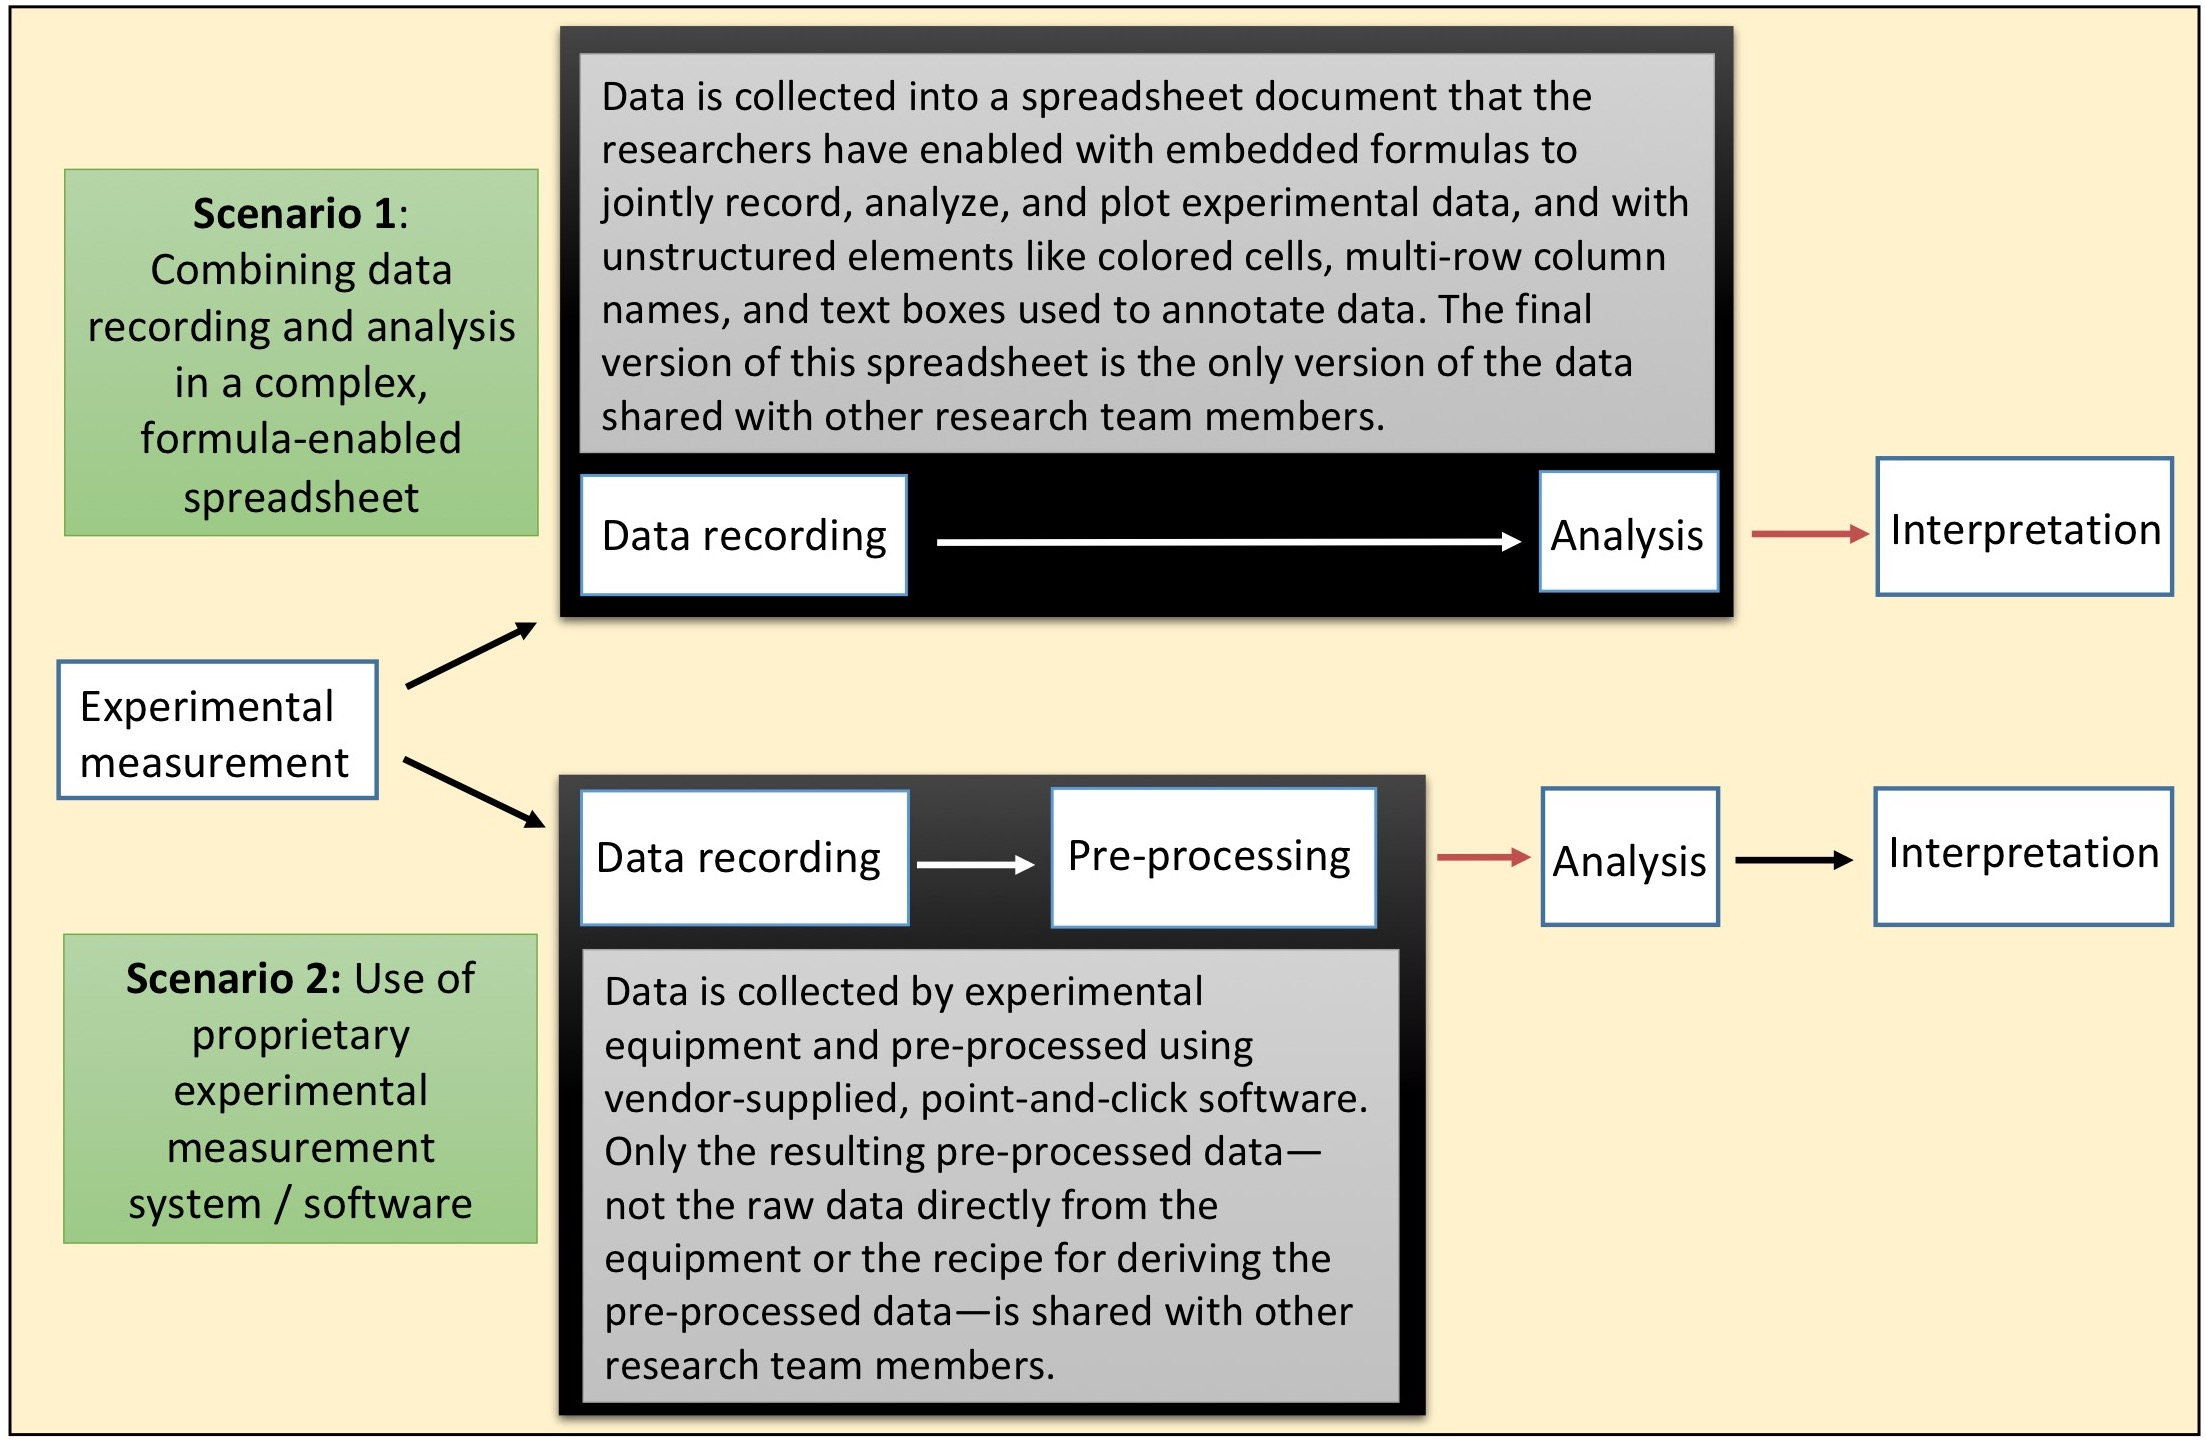
\includegraphics[width=30.64in]{figures/existing_blackboxes} 

}

\caption[Two scenarios where 'black boxes' of non-transparent, non-reproducible data handling exist in research data workflows at the stages of data recording and pre-processing]{Two scenarios where 'black boxes' of non-transparent, non-reproducible data handling exist in research data workflows at the stages of data recording and pre-processing. These create potential points of failure for reproducible research. Red arrows indicate where data is passed to other research team members, including statisticians / data analysts, often within complex or unstructured spreadsheet files.}\label{fig:workflow}
\end{figure*}

It is widely known and discussed among data scientists, mathematical modelers,
and statisticians \citep{broman2018data, krishnan2016towards} that there is
frequently a need to discard, transform, and reformat various elements of the
data shared with them by laboratory-based researchers, and that data is often
shared in an unstructured format, increasing the risks of introducing errors
through reformatting before applying more advanced computational methods.
Instead, a critical need for reproducibility is for the transparent and clear
sharing across research teams of: (1) raw data, directly from hand-recording or
directly output from experimental equipment; (2) data that has been
pre-processed as necessary (e.g., gating for flow cytometry data, feature
identification for metabolomics data), saved in a consistent, structured format,
and (3) a clear and repeatable description of how the pre-processed data was
generated from the raw data \citep{broman2018data, ellis2018share}.

To enhance data reproducibility, it is critical to create a clear separation
among data recording, data pre-processing, and data analysis---breaking up
commonly existing ``black boxes" in data handling across the research process.
Such a rigorous demarcation requires some change in the conventional
understanding and use of spreadsheets and a recognition by biomedical
researchers that recent advances in computer programming languages, especially
the R programming language, provide user-friendly and accessible tools and
concepts that can be used to extend a transparent and reproducible data workflow
to the steps of data recording and pre-processing. Among our team, we have found
that there are many common existing practices---including use of spreadsheets
with embedded formulas that concurrently record and analyze experimental data,
problematic management of project files, and reliance on proprietary,
vendor-supplied point-and-click software for data pre-processing---that can
interfere with the transparency, reproducibility, and efficiency of
laboratory-based biomedical research projects, problems that have also been
identified by others as key barriers to research reproducibility
\citep[ \citet{marwick2018packaging}]{broman2018data, bryan2018excuse, ellis2018share}. In
these training modules, we have choosen topics that tackle barriers to
reproducibility that have straightforward, easy-to-teach solutions, but which
are still very common in biomedical laboratory-based research programs.

\hypertarget{license}{%
\section{License}\label{license}}

This book is licensed under the \href{https://creativecommons.org/licenses/by-nc-sa/4.0/}{Creative Commons
Attribution-NonCommercial-ShareAlike 4.0 International
License}, while all code in
the book is under the \href{https://opensource.org/licenses/MIT}{MIT license}.

Click on the \textbf{Next} button (or navigate using the
links at the top of the page) to continue.

\hypertarget{experimental-data-recording}{%
\chapter{Experimental Data Recording}\label{experimental-data-recording}}

\hypertarget{separating-data-recording-and-analysis}{%
\section{Separating data recording and analysis}\label{separating-data-recording-and-analysis}}

Many biomedical laboratories use spreadsheets, with embedded formulas, to both
record and analyze experimental data. This practice impedes transparency and
reproducibility of both data recording and data analysis. In this module, we
will describe this common practice and will outline alternative approaches that
separate the steps of data recording and data analysis.

\textbf{Objectives.} After this module, the trainee will be able to:

\begin{itemize}
\tightlist
\item
  Explain the difference between data recording and data analysis
\item
  Understand why collecting data on spreadsheets with embedded formulas impedes
  reproducibility
\item
  List alternative approaches to improve reproducibility
\end{itemize}

\hypertarget{data-recording-versus-data-analysis}{%
\subsection{Data recording versus data analysis}\label{data-recording-versus-data-analysis}}

\hypertarget{common-practices-combining-recording-and-analysis}{%
\subsection{Common practices combining recording and analysis}\label{common-practices-combining-recording-and-analysis}}

\hypertarget{hazards-of-combining-recording-and-analysis}{%
\subsection{Hazards of combining recording and analysis}\label{hazards-of-combining-recording-and-analysis}}

\hypertarget{approaches-to-separate-recording-and-analysis}{%
\subsection{Approaches to separate recording and analysis}\label{approaches-to-separate-recording-and-analysis}}

\hypertarget{discussion-questions}{%
\subsection{Discussion questions}\label{discussion-questions}}

\hypertarget{principles-and-power-of-structured-data-formats}{%
\section{Principles and power of structured data formats}\label{principles-and-power-of-structured-data-formats}}

The format in which experimental data is recorded can have a large influence on
how easy and likely it is to implement reproducibility tools in later stages of
the research workflow. Recording data in a ``structured'' format brings many
benefits. In this module, we will explain what makes a dataset ``structured'' and
why this format is a powerful tool for reproducible research.

\textbf{Objectives.} After this module, the trainee will be able to:

\begin{itemize}
\tightlist
\item
  List the characteristics of a structured data format
\item
  Describe benefits for research transparency and reproducibility
\item
  Outline other benefits of using a structured format when recording data
\end{itemize}

\hypertarget{characteristics-of-a-structured-data-format}{%
\subsection{Characteristics of a structured data format}\label{characteristics-of-a-structured-data-format}}

\hypertarget{benefits-of-a-structured-data-format}{%
\subsection{Benefits of a structured data format}\label{benefits-of-a-structured-data-format}}

\hypertarget{applied-exercise}{%
\subsection{Applied exercise}\label{applied-exercise}}

\hypertarget{the-tidy-data-format}{%
\section{The `tidy' data format}\label{the-tidy-data-format}}

The ``tidy'' data format is an implementation of a structured data format popular
among statisticians and data scientists. By consistently using this data format,
researchers can combine simple, generalizable tools to perform complex tasks in
data processing, analysis, and visualization. We will explain what
characteristics determine if a dataset is ``tidy'' and how use of the ``tidy''
implementation of a structure data format can improve the ease and efficiency of
``Team Science''.

\textbf{Objectives.} After this module, the trainee will be able to:

\begin{itemize}
\tightlist
\item
  List characteristics defining the ``tidy'' structured data format
\item
  Explain the difference between the a structured data format (general concept)
  and the `tidy' data format (one popular implementation)
\end{itemize}

\hypertarget{the-tidy-data-format-1}{%
\subsection{The ``tidy'' data format}\label{the-tidy-data-format-1}}

\hypertarget{the-tidy-data-format-as-a-structured-data-format}{%
\subsection{The ``tidy'' data format as a structured data format}\label{the-tidy-data-format-as-a-structured-data-format}}

\hypertarget{practice-quiz}{%
\subsection{Practice quiz}\label{practice-quiz}}

\hypertarget{designing-templates-for-tidy-data-collection}{%
\section{Designing templates for ``tidy'' data collection}\label{designing-templates-for-tidy-data-collection}}

This module will move from the principles of the ``tidy'' data format to the
practical details of designing a ``tidy'' data format to use when collecting
experimental data. We will describe common issues that prevent biomedical
research datasets from being ``tidy'' and show how these issues can be avoided. We
will also provide rubrics and a checklist to help determine if a data collection
template complies with a ``tidy'' format.

\textbf{Objectives.} After this module, the trainee will be able to:

\begin{itemize}
\tightlist
\item
  Identify characteristics that keep a dataset from being `tidy'
\item
  Convert data from an ``untidy'' to a ``tidy'' format
\end{itemize}

\hypertarget{subsection-1}{%
\subsection{Subsection 1}\label{subsection-1}}

\hypertarget{applied-exercise-1}{%
\subsection{Applied exercise}\label{applied-exercise-1}}

\hypertarget{separating-data-recording-and-analysis-1}{%
\section{Separating data recording and analysis}\label{separating-data-recording-and-analysis-1}}

Many biomedical laboratories use spreadsheets, with embedded formulas, to both
record and analyze experimental data. This practice impedes transparency and
reproducibility of both data recording and data analysis. In this module, we
will describe this common practice and will outline alternative approaches that
separate the steps of data recording and data analysis.

\textbf{Objectives.} After this module, the trainee will be able to:

\begin{itemize}
\tightlist
\item
  Explain the difference between data recording and data analysis
\item
  Understand why collecting data on spreadsheets with embedded formulas impedes
  reproducibility
\item
  List alternative approaches to improve reproducibility
\end{itemize}

\hypertarget{data-recording-versus-data-analysis-1}{%
\subsection{Data recording versus data analysis}\label{data-recording-versus-data-analysis-1}}

\hypertarget{common-practices-combining-recording-and-analysis-1}{%
\subsection{Common practices combining recording and analysis}\label{common-practices-combining-recording-and-analysis-1}}

\hypertarget{hazards-of-combining-recording-and-analysis-1}{%
\subsection{Hazards of combining recording and analysis}\label{hazards-of-combining-recording-and-analysis-1}}

\hypertarget{approaches-to-separate-recording-and-analysis-1}{%
\subsection{Approaches to separate recording and analysis}\label{approaches-to-separate-recording-and-analysis-1}}

\hypertarget{discussion-questions-1}{%
\subsection{Discussion questions}\label{discussion-questions-1}}

\hypertarget{separating-data-recording-and-analysis-2}{%
\section{Separating data recording and analysis}\label{separating-data-recording-and-analysis-2}}

Many biomedical laboratories use spreadsheets, with embedded formulas, to both
record and analyze experimental data. This practice impedes transparency and
reproducibility of both data recording and data analysis. In this module, we
will describe this common practice and will outline alternative approaches that
separate the steps of data recording and data analysis.

\textbf{Objectives.} After this module, the trainee will be able to:

\begin{itemize}
\tightlist
\item
  Explain the difference between data recording and data analysis
\item
  Understand why collecting data on spreadsheets with embedded formulas impedes
  reproducibility
\item
  List alternative approaches to improve reproducibility
\end{itemize}

\hypertarget{data-recording-versus-data-analysis-2}{%
\subsection{Data recording versus data analysis}\label{data-recording-versus-data-analysis-2}}

\hypertarget{common-practices-combining-recording-and-analysis-2}{%
\subsection{Common practices combining recording and analysis}\label{common-practices-combining-recording-and-analysis-2}}

\hypertarget{hazards-of-combining-recording-and-analysis-2}{%
\subsection{Hazards of combining recording and analysis}\label{hazards-of-combining-recording-and-analysis-2}}

\hypertarget{approaches-to-separate-recording-and-analysis-2}{%
\subsection{Approaches to separate recording and analysis}\label{approaches-to-separate-recording-and-analysis-2}}

\hypertarget{discussion-questions-2}{%
\subsection{Discussion questions}\label{discussion-questions-2}}

\hypertarget{separating-data-recording-and-analysis-3}{%
\section{Separating data recording and analysis}\label{separating-data-recording-and-analysis-3}}

Many biomedical laboratories use spreadsheets, with embedded formulas, to both
record and analyze experimental data. This practice impedes transparency and
reproducibility of both data recording and data analysis. In this module, we
will describe this common practice and will outline alternative approaches that
separate the steps of data recording and data analysis.

\textbf{Objectives.} After this module, the trainee will be able to:

\begin{itemize}
\tightlist
\item
  Explain the difference between data recording and data analysis
\item
  Understand why collecting data on spreadsheets with embedded formulas impedes
  reproducibility
\item
  List alternative approaches to improve reproducibility
\end{itemize}

\hypertarget{data-recording-versus-data-analysis-3}{%
\subsection{Data recording versus data analysis}\label{data-recording-versus-data-analysis-3}}

\hypertarget{common-practices-combining-recording-and-analysis-3}{%
\subsection{Common practices combining recording and analysis}\label{common-practices-combining-recording-and-analysis-3}}

\hypertarget{hazards-of-combining-recording-and-analysis-3}{%
\subsection{Hazards of combining recording and analysis}\label{hazards-of-combining-recording-and-analysis-3}}

\hypertarget{approaches-to-separate-recording-and-analysis-3}{%
\subsection{Approaches to separate recording and analysis}\label{approaches-to-separate-recording-and-analysis-3}}

\hypertarget{discussion-questions-3}{%
\subsection{Discussion questions}\label{discussion-questions-3}}

\hypertarget{separating-data-recording-and-analysis-4}{%
\section{Separating data recording and analysis}\label{separating-data-recording-and-analysis-4}}

Many biomedical laboratories use spreadsheets, with embedded formulas, to both
record and analyze experimental data. This practice impedes transparency and
reproducibility of both data recording and data analysis. In this module, we
will describe this common practice and will outline alternative approaches that
separate the steps of data recording and data analysis.

\textbf{Objectives.} After this module, the trainee will be able to:

\begin{itemize}
\tightlist
\item
  Explain the difference between data recording and data analysis
\item
  Understand why collecting data on spreadsheets with embedded formulas impedes
  reproducibility
\item
  List alternative approaches to improve reproducibility
\end{itemize}

\hypertarget{data-recording-versus-data-analysis-4}{%
\subsection{Data recording versus data analysis}\label{data-recording-versus-data-analysis-4}}

\hypertarget{common-practices-combining-recording-and-analysis-4}{%
\subsection{Common practices combining recording and analysis}\label{common-practices-combining-recording-and-analysis-4}}

\hypertarget{hazards-of-combining-recording-and-analysis-4}{%
\subsection{Hazards of combining recording and analysis}\label{hazards-of-combining-recording-and-analysis-4}}

\hypertarget{approaches-to-separate-recording-and-analysis-4}{%
\subsection{Approaches to separate recording and analysis}\label{approaches-to-separate-recording-and-analysis-4}}

\hypertarget{discussion-questions-4}{%
\subsection{Discussion questions}\label{discussion-questions-4}}

\hypertarget{separating-data-recording-and-analysis-5}{%
\section{Separating data recording and analysis}\label{separating-data-recording-and-analysis-5}}

Many biomedical laboratories use spreadsheets, with embedded formulas, to both
record and analyze experimental data. This practice impedes transparency and
reproducibility of both data recording and data analysis. In this module, we
will describe this common practice and will outline alternative approaches that
separate the steps of data recording and data analysis.

\textbf{Objectives.} After this module, the trainee will be able to:

\begin{itemize}
\tightlist
\item
  Explain the difference between data recording and data analysis
\item
  Understand why collecting data on spreadsheets with embedded formulas impedes
  reproducibility
\item
  List alternative approaches to improve reproducibility
\end{itemize}

\hypertarget{data-recording-versus-data-analysis-5}{%
\subsection{Data recording versus data analysis}\label{data-recording-versus-data-analysis-5}}

\hypertarget{common-practices-combining-recording-and-analysis-5}{%
\subsection{Common practices combining recording and analysis}\label{common-practices-combining-recording-and-analysis-5}}

\hypertarget{hazards-of-combining-recording-and-analysis-5}{%
\subsection{Hazards of combining recording and analysis}\label{hazards-of-combining-recording-and-analysis-5}}

\hypertarget{approaches-to-separate-recording-and-analysis-5}{%
\subsection{Approaches to separate recording and analysis}\label{approaches-to-separate-recording-and-analysis-5}}

\hypertarget{discussion-questions-5}{%
\subsection{Discussion questions}\label{discussion-questions-5}}

\hypertarget{separating-data-recording-and-analysis-6}{%
\section{Separating data recording and analysis}\label{separating-data-recording-and-analysis-6}}

Many biomedical laboratories use spreadsheets, with embedded formulas, to both
record and analyze experimental data. This practice impedes transparency and
reproducibility of both data recording and data analysis. In this module, we
will describe this common practice and will outline alternative approaches that
separate the steps of data recording and data analysis.

\textbf{Objectives.} After this module, the trainee will be able to:

\begin{itemize}
\tightlist
\item
  Explain the difference between data recording and data analysis
\item
  Understand why collecting data on spreadsheets with embedded formulas impedes
  reproducibility
\item
  List alternative approaches to improve reproducibility
\end{itemize}

\hypertarget{data-recording-versus-data-analysis-6}{%
\subsection{Data recording versus data analysis}\label{data-recording-versus-data-analysis-6}}

\hypertarget{common-practices-combining-recording-and-analysis-6}{%
\subsection{Common practices combining recording and analysis}\label{common-practices-combining-recording-and-analysis-6}}

\hypertarget{hazards-of-combining-recording-and-analysis-6}{%
\subsection{Hazards of combining recording and analysis}\label{hazards-of-combining-recording-and-analysis-6}}

\hypertarget{approaches-to-separate-recording-and-analysis-6}{%
\subsection{Approaches to separate recording and analysis}\label{approaches-to-separate-recording-and-analysis-6}}

\hypertarget{discussion-questions-6}{%
\subsection{Discussion questions}\label{discussion-questions-6}}

\hypertarget{separating-data-recording-and-analysis-7}{%
\section{Separating data recording and analysis}\label{separating-data-recording-and-analysis-7}}

Many biomedical laboratories use spreadsheets, with embedded formulas, to both
record and analyze experimental data. This practice impedes transparency and
reproducibility of both data recording and data analysis. In this module, we
will describe this common practice and will outline alternative approaches that
separate the steps of data recording and data analysis.

\textbf{Objectives.} After this module, the trainee will be able to:

\begin{itemize}
\tightlist
\item
  Explain the difference between data recording and data analysis
\item
  Understand why collecting data on spreadsheets with embedded formulas impedes
  reproducibility
\item
  List alternative approaches to improve reproducibility
\end{itemize}

\hypertarget{data-recording-versus-data-analysis-7}{%
\subsection{Data recording versus data analysis}\label{data-recording-versus-data-analysis-7}}

\hypertarget{common-practices-combining-recording-and-analysis-7}{%
\subsection{Common practices combining recording and analysis}\label{common-practices-combining-recording-and-analysis-7}}

\hypertarget{hazards-of-combining-recording-and-analysis-7}{%
\subsection{Hazards of combining recording and analysis}\label{hazards-of-combining-recording-and-analysis-7}}

\hypertarget{approaches-to-separate-recording-and-analysis-7}{%
\subsection{Approaches to separate recording and analysis}\label{approaches-to-separate-recording-and-analysis-7}}

\hypertarget{discussion-questions-7}{%
\subsection{Discussion questions}\label{discussion-questions-7}}

\hypertarget{experimental-data-preprocessing}{%
\chapter{Experimental Data Preprocessing}\label{experimental-data-preprocessing}}

\hypertarget{separating-data-recording-and-analysis-8}{%
\section{Separating data recording and analysis}\label{separating-data-recording-and-analysis-8}}

Many biomedical laboratories use spreadsheets, with embedded formulas, to both
record and analyze experimental data. This practice impedes transparency and
reproducibility of both data recording and data analysis. In this module, we
will describe this common practice and will outline alternative approaches that
separate the steps of data recording and data analysis.

\textbf{Objectives.} After this module, the trainee will be able to:

\begin{itemize}
\tightlist
\item
  Explain the difference between data recording and data analysis
\item
  Understand why collecting data on spreadsheets with embedded formulas impedes
  reproducibility
\item
  List alternative approaches to improve reproducibility
\end{itemize}

\hypertarget{data-recording-versus-data-analysis-8}{%
\subsection{Data recording versus data analysis}\label{data-recording-versus-data-analysis-8}}

\hypertarget{common-practices-combining-recording-and-analysis-8}{%
\subsection{Common practices combining recording and analysis}\label{common-practices-combining-recording-and-analysis-8}}

\hypertarget{hazards-of-combining-recording-and-analysis-8}{%
\subsection{Hazards of combining recording and analysis}\label{hazards-of-combining-recording-and-analysis-8}}

\hypertarget{approaches-to-separate-recording-and-analysis-8}{%
\subsection{Approaches to separate recording and analysis}\label{approaches-to-separate-recording-and-analysis-8}}

\hypertarget{discussion-questions-8}{%
\subsection{Discussion questions}\label{discussion-questions-8}}

\hypertarget{separating-data-recording-and-analysis-9}{%
\section{Separating data recording and analysis}\label{separating-data-recording-and-analysis-9}}

Many biomedical laboratories use spreadsheets, with embedded formulas, to both
record and analyze experimental data. This practice impedes transparency and
reproducibility of both data recording and data analysis. In this module, we
will describe this common practice and will outline alternative approaches that
separate the steps of data recording and data analysis.

\textbf{Objectives.} After this module, the trainee will be able to:

\begin{itemize}
\tightlist
\item
  Explain the difference between data recording and data analysis
\item
  Understand why collecting data on spreadsheets with embedded formulas impedes
  reproducibility
\item
  List alternative approaches to improve reproducibility
\end{itemize}

\hypertarget{data-recording-versus-data-analysis-9}{%
\subsection{Data recording versus data analysis}\label{data-recording-versus-data-analysis-9}}

\hypertarget{common-practices-combining-recording-and-analysis-9}{%
\subsection{Common practices combining recording and analysis}\label{common-practices-combining-recording-and-analysis-9}}

\hypertarget{hazards-of-combining-recording-and-analysis-9}{%
\subsection{Hazards of combining recording and analysis}\label{hazards-of-combining-recording-and-analysis-9}}

\hypertarget{approaches-to-separate-recording-and-analysis-9}{%
\subsection{Approaches to separate recording and analysis}\label{approaches-to-separate-recording-and-analysis-9}}

\hypertarget{discussion-questions-9}{%
\subsection{Discussion questions}\label{discussion-questions-9}}

\hypertarget{separating-data-recording-and-analysis-10}{%
\section{Separating data recording and analysis}\label{separating-data-recording-and-analysis-10}}

Many biomedical laboratories use spreadsheets, with embedded formulas, to both
record and analyze experimental data. This practice impedes transparency and
reproducibility of both data recording and data analysis. In this module, we
will describe this common practice and will outline alternative approaches that
separate the steps of data recording and data analysis.

\textbf{Objectives.} After this module, the trainee will be able to:

\begin{itemize}
\tightlist
\item
  Explain the difference between data recording and data analysis
\item
  Understand why collecting data on spreadsheets with embedded formulas impedes
  reproducibility
\item
  List alternative approaches to improve reproducibility
\end{itemize}

\hypertarget{data-recording-versus-data-analysis-10}{%
\subsection{Data recording versus data analysis}\label{data-recording-versus-data-analysis-10}}

\hypertarget{common-practices-combining-recording-and-analysis-10}{%
\subsection{Common practices combining recording and analysis}\label{common-practices-combining-recording-and-analysis-10}}

\hypertarget{hazards-of-combining-recording-and-analysis-10}{%
\subsection{Hazards of combining recording and analysis}\label{hazards-of-combining-recording-and-analysis-10}}

\hypertarget{approaches-to-separate-recording-and-analysis-10}{%
\subsection{Approaches to separate recording and analysis}\label{approaches-to-separate-recording-and-analysis-10}}

\hypertarget{discussion-questions-10}{%
\subsection{Discussion questions}\label{discussion-questions-10}}

\hypertarget{separating-data-recording-and-analysis-11}{%
\section{Separating data recording and analysis}\label{separating-data-recording-and-analysis-11}}

Many biomedical laboratories use spreadsheets, with embedded formulas, to both
record and analyze experimental data. This practice impedes transparency and
reproducibility of both data recording and data analysis. In this module, we
will describe this common practice and will outline alternative approaches that
separate the steps of data recording and data analysis.

\textbf{Objectives.} After this module, the trainee will be able to:

\begin{itemize}
\tightlist
\item
  Explain the difference between data recording and data analysis
\item
  Understand why collecting data on spreadsheets with embedded formulas impedes
  reproducibility
\item
  List alternative approaches to improve reproducibility
\end{itemize}

\hypertarget{data-recording-versus-data-analysis-11}{%
\subsection{Data recording versus data analysis}\label{data-recording-versus-data-analysis-11}}

\hypertarget{common-practices-combining-recording-and-analysis-11}{%
\subsection{Common practices combining recording and analysis}\label{common-practices-combining-recording-and-analysis-11}}

\hypertarget{hazards-of-combining-recording-and-analysis-11}{%
\subsection{Hazards of combining recording and analysis}\label{hazards-of-combining-recording-and-analysis-11}}

\hypertarget{approaches-to-separate-recording-and-analysis-11}{%
\subsection{Approaches to separate recording and analysis}\label{approaches-to-separate-recording-and-analysis-11}}

\hypertarget{discussion-questions-11}{%
\subsection{Discussion questions}\label{discussion-questions-11}}

\hypertarget{separating-data-recording-and-analysis-12}{%
\section{Separating data recording and analysis}\label{separating-data-recording-and-analysis-12}}

Many biomedical laboratories use spreadsheets, with embedded formulas, to both
record and analyze experimental data. This practice impedes transparency and
reproducibility of both data recording and data analysis. In this module, we
will describe this common practice and will outline alternative approaches that
separate the steps of data recording and data analysis.

\textbf{Objectives.} After this module, the trainee will be able to:

\begin{itemize}
\tightlist
\item
  Explain the difference between data recording and data analysis
\item
  Understand why collecting data on spreadsheets with embedded formulas impedes
  reproducibility
\item
  List alternative approaches to improve reproducibility
\end{itemize}

\hypertarget{data-recording-versus-data-analysis-12}{%
\subsection{Data recording versus data analysis}\label{data-recording-versus-data-analysis-12}}

\hypertarget{common-practices-combining-recording-and-analysis-12}{%
\subsection{Common practices combining recording and analysis}\label{common-practices-combining-recording-and-analysis-12}}

\hypertarget{hazards-of-combining-recording-and-analysis-12}{%
\subsection{Hazards of combining recording and analysis}\label{hazards-of-combining-recording-and-analysis-12}}

\hypertarget{approaches-to-separate-recording-and-analysis-12}{%
\subsection{Approaches to separate recording and analysis}\label{approaches-to-separate-recording-and-analysis-12}}

\hypertarget{discussion-questions-12}{%
\subsection{Discussion questions}\label{discussion-questions-12}}

\hypertarget{separating-data-recording-and-analysis-13}{%
\section{Separating data recording and analysis}\label{separating-data-recording-and-analysis-13}}

Many biomedical laboratories use spreadsheets, with embedded formulas, to both
record and analyze experimental data. This practice impedes transparency and
reproducibility of both data recording and data analysis. In this module, we
will describe this common practice and will outline alternative approaches that
separate the steps of data recording and data analysis.

\textbf{Objectives.} After this module, the trainee will be able to:

\begin{itemize}
\tightlist
\item
  Explain the difference between data recording and data analysis
\item
  Understand why collecting data on spreadsheets with embedded formulas impedes
  reproducibility
\item
  List alternative approaches to improve reproducibility
\end{itemize}

\hypertarget{data-recording-versus-data-analysis-13}{%
\subsection{Data recording versus data analysis}\label{data-recording-versus-data-analysis-13}}

\hypertarget{common-practices-combining-recording-and-analysis-13}{%
\subsection{Common practices combining recording and analysis}\label{common-practices-combining-recording-and-analysis-13}}

\hypertarget{hazards-of-combining-recording-and-analysis-13}{%
\subsection{Hazards of combining recording and analysis}\label{hazards-of-combining-recording-and-analysis-13}}

\hypertarget{approaches-to-separate-recording-and-analysis-13}{%
\subsection{Approaches to separate recording and analysis}\label{approaches-to-separate-recording-and-analysis-13}}

\hypertarget{discussion-questions-13}{%
\subsection{Discussion questions}\label{discussion-questions-13}}

\hypertarget{separating-data-recording-and-analysis-14}{%
\section{Separating data recording and analysis}\label{separating-data-recording-and-analysis-14}}

Many biomedical laboratories use spreadsheets, with embedded formulas, to both
record and analyze experimental data. This practice impedes transparency and
reproducibility of both data recording and data analysis. In this module, we
will describe this common practice and will outline alternative approaches that
separate the steps of data recording and data analysis.

\textbf{Objectives.} After this module, the trainee will be able to:

\begin{itemize}
\tightlist
\item
  Explain the difference between data recording and data analysis
\item
  Understand why collecting data on spreadsheets with embedded formulas impedes
  reproducibility
\item
  List alternative approaches to improve reproducibility
\end{itemize}

\hypertarget{data-recording-versus-data-analysis-14}{%
\subsection{Data recording versus data analysis}\label{data-recording-versus-data-analysis-14}}

\hypertarget{common-practices-combining-recording-and-analysis-14}{%
\subsection{Common practices combining recording and analysis}\label{common-practices-combining-recording-and-analysis-14}}

\hypertarget{hazards-of-combining-recording-and-analysis-14}{%
\subsection{Hazards of combining recording and analysis}\label{hazards-of-combining-recording-and-analysis-14}}

\hypertarget{approaches-to-separate-recording-and-analysis-14}{%
\subsection{Approaches to separate recording and analysis}\label{approaches-to-separate-recording-and-analysis-14}}

\hypertarget{discussion-questions-14}{%
\subsection{Discussion questions}\label{discussion-questions-14}}

\hypertarget{separating-data-recording-and-analysis-15}{%
\section{Separating data recording and analysis}\label{separating-data-recording-and-analysis-15}}

Many biomedical laboratories use spreadsheets, with embedded formulas, to both
record and analyze experimental data. This practice impedes transparency and
reproducibility of both data recording and data analysis. In this module, we
will describe this common practice and will outline alternative approaches that
separate the steps of data recording and data analysis.

\textbf{Objectives.} After this module, the trainee will be able to:

\begin{itemize}
\tightlist
\item
  Explain the difference between data recording and data analysis
\item
  Understand why collecting data on spreadsheets with embedded formulas impedes
  reproducibility
\item
  List alternative approaches to improve reproducibility
\end{itemize}

\hypertarget{data-recording-versus-data-analysis-15}{%
\subsection{Data recording versus data analysis}\label{data-recording-versus-data-analysis-15}}

\hypertarget{common-practices-combining-recording-and-analysis-15}{%
\subsection{Common practices combining recording and analysis}\label{common-practices-combining-recording-and-analysis-15}}

\hypertarget{hazards-of-combining-recording-and-analysis-15}{%
\subsection{Hazards of combining recording and analysis}\label{hazards-of-combining-recording-and-analysis-15}}

\hypertarget{approaches-to-separate-recording-and-analysis-15}{%
\subsection{Approaches to separate recording and analysis}\label{approaches-to-separate-recording-and-analysis-15}}

\hypertarget{discussion-questions-15}{%
\subsection{Discussion questions}\label{discussion-questions-15}}

\hypertarget{separating-data-recording-and-analysis-16}{%
\section{Separating data recording and analysis}\label{separating-data-recording-and-analysis-16}}

Many biomedical laboratories use spreadsheets, with embedded formulas, to both
record and analyze experimental data. This practice impedes transparency and
reproducibility of both data recording and data analysis. In this module, we
will describe this common practice and will outline alternative approaches that
separate the steps of data recording and data analysis.

\textbf{Objectives.} After this module, the trainee will be able to:

\begin{itemize}
\tightlist
\item
  Explain the difference between data recording and data analysis
\item
  Understand why collecting data on spreadsheets with embedded formulas impedes
  reproducibility
\item
  List alternative approaches to improve reproducibility
\end{itemize}

\hypertarget{data-recording-versus-data-analysis-16}{%
\subsection{Data recording versus data analysis}\label{data-recording-versus-data-analysis-16}}

\hypertarget{common-practices-combining-recording-and-analysis-16}{%
\subsection{Common practices combining recording and analysis}\label{common-practices-combining-recording-and-analysis-16}}

\hypertarget{hazards-of-combining-recording-and-analysis-16}{%
\subsection{Hazards of combining recording and analysis}\label{hazards-of-combining-recording-and-analysis-16}}

\hypertarget{approaches-to-separate-recording-and-analysis-16}{%
\subsection{Approaches to separate recording and analysis}\label{approaches-to-separate-recording-and-analysis-16}}

\hypertarget{discussion-questions-16}{%
\subsection{Discussion questions}\label{discussion-questions-16}}

\bibliography{book.bib,packages.bib}



\end{document}
